\documentclass[11pt]{article}

\usepackage{amsmath,amssymb}
\usepackage{clrscode3e}
\usepackage{color}
\usepackage{epigraph}
\usepackage{fourier}
\usepackage{euler}
\usepackage{fullpage}
\usepackage{fullpage}
\usepackage{graphicx}
\usepackage[colorlinks=true,urlcolor=blue]{hyperref}
\usepackage{listings}
\usepackage{url}
\usepackage{xspace}
\usepackage[shortlabels]{enumitem}

\usepackage{fancyhdr}
\pagestyle{fancy}
\fancyhf{}

\fancypagestyle{plain}{%
  \fancyhf{}
  \renewcommand{\headrulewidth}{0pt}
  \renewcommand{\footrulewidth}{0pt}
  \lfoot{\textcopyright{} 2021 Darrell Long}
  \rfoot{\thepage}
}

\pagestyle{plain}

\newenvironment{funcdoc}[1]{\subsubsection*{\underline{\textbf{\texttt{#1}}}}}{}

\definecolor{codegreen}{rgb}{0,0.5,0}
\definecolor{codegray}{rgb}{0.5,0.5,0.5}
\definecolor{codepurple}{rgb}{0.58,0,0.82}

\lstloadlanguages{C,make,python,fortran}

\lstdefinestyle{c99}{
    morekeywords={bool, uint8_t, uint16_t, uint32_t, uint64_t, int8_t, int16_t, int32_t, int64_t},
    commentstyle=\color{codegreen},
    keywordstyle=\color{magenta},
    numberstyle=\tiny\color{codegray},
    identifierstyle=\color{blue},
    stringstyle=\color{codepurple},
    basicstyle=\ttfamily,
    breakatwhitespace=false,
    breaklines=true,
    captionpos=b,
    keepspaces=true,
    numbers=left,
    numbersep=5pt,
    showspaces=false,
    showstringspaces=false,
    showtabs=false,
    tabsize=4
}

\newcommand{\monkey}[1]{
  \begin{center}
    
\includegraphics[width=0.35\textwidth]{../monkey.jpg} \\
    \emph{#1}
  \end{center}
}


\title{Assignment 6 \\ Public Key Cryptography}
\author{
  Prof.\xspace Darrell D.\xspace E.\xspace Long \\
  CSE 13S -- Fall 2021
}
\date{
  First \texttt{DESIGN.pdf} draft due: November 11$^\text{th}$ at 11:59\,pm PST \\
  Assignment due: November 21$^\text{st}$ at 11:59\,pm PST
}

\begin{document}

\maketitle

\section{Introduction}

\epigraphwidth=0.75\textwidth
\epigraph{\emph{Doo Jdxo lv glylghg lqwr wkuhh sduwv, rqh ri zklfk wkh Ehojdh lqkdelw, wkh Dtxlwdql dqrwkhu, wkrvh zkr lq wkhlu rzq odqjxdjh duh fdoohg Fhowv, lq rxu Jdxov, wkh wklug.}}{---Julius C{\ae}sar}

\noindent
Cryptography, once restricted to government, spies, and the military is
now pervasive in our lives. Most web sites that you visit are protected
using SSL. Your SSH connections are protected in the same way.

How is this accomplished? Through a mixture of \emph{public key} and
\emph{symmetric key} cryptography. The earliest known practical
public-key cryptography algorithm is RSA, after its inventors Ronald
Rivest, Adi Shamir, and Leonard Adleman (Figure\xspace\ref{fig:rsa}),
who published it in 1978. About
five years earlier, on 20 November, 1973, Clifford Cocks (Figure\xspace\ref{fig:cocks}), working for
GCHQ (the British equivalent of the NSA), invented a very similar
algorithm. His classified memorandum ``A note on `non-secret'
encryption'' was to remain secret for 24 years. In fact, when you read
the Cocks memorandum, you will see that the \emph{idea} of public key
encryption was proposed by J.\xspace H.\xspace Ellis three years earlier
in 1970. Unknown in the public literature, the idea was independently
proposed by Ralph Merkle for public key distribution, which inspired
asymmetric cryptography by  Whitfield Diffie and Martin Hellman, and
finally leading to RSA.

Public-key cryptography, or asymmetric cryptography, is a cryptographic
system that uses pairs of keys: public keys (known to others) and
private keys (known only by the owner). The generation of such key pairs
depends on cryptographic algorithms that are based on mathematical
objects called \emph{one-way functions}. Security requires keeping the
private key private; the public key can be distributed widely.

Any person can encrypt a message using the intended receiver's public
key, but that encrypted message can only be decrypted with the
receiver's private key. This allows a server to create a cryptographic
key for suitable symmetric-key cryptography and then use a client's
openly shared public key to encrypt the newly generated symmetric key.
The server can then send this encrypted symmetric key over an insecure
channel to the client; only the client can decrypt it using its private
key. With the client and server both having the same symmetric key, they
can safely use symmetric key encryption to communicate. This scheme has
the advantage of not having to pre-share symmetric keys while gaining the
higher speed of symmetric-key cryptography.

Symmetric-key algorithms use the same cryptographic keys for the
encryption of plaintext and the decryption of ciphertext. The keys may
be identical, or there may be a simple transformation between the two
keys. The keys represent a shared secret between two or more parties.
The requirement that both parties have access to the secret key is one
of the main disadvantages of symmetric-key encryption compared to
public-key encryption.

Let's briefly look at the Cocks algorithm before moving on to the more
popular RSA algorithm.  We have two principals: \emph{Alice} ($A$), who is
the receiver, and \emph{Bonnie} ($B$), who is the sender.

\begin{enumerate}[(a)]
  \item Alice:
  \begin{enumerate}[i.]
    \item Chooses two primes $p$ and $q$ such that $p \nmid (q-1)$ and $q
    \nmid (p-1)$. That is, $p$ does not divide $q-1$ and $q$ does not
      divide $p -1$.
    \item Transmits the computed product $n = p q$ to the sender, which we
      write as $A \xrightarrow{n} B$.
  \end{enumerate}
  \item Bonnie:
  \begin{enumerate}[i.]
    \item Has a message consisting of numbers $c_1, c_2, \ldots, c_r$
      where $0 < c_i < n$.
    \item Sends these encoded as $d_i$ where $d_i = c_i^n \pmod{n}$.
      When written as part of a protocol, $B \xrightarrow{c_1, \ldots,
      c_r} A$.
  \end{enumerate}
  \item Alice:
  \begin{enumerate}[i.]
    \item Computes using Euclid's Algorithm $p^\prime$ such that
      $p\times p^\prime \equiv 1 \pmod{q-1}$, and $q^\prime$ such that
      $q\times q^\prime \equiv 1 \pmod{p-1}$.
    \item Decodes $c_i = d_i^{p^\prime} \pmod{q} = d_i^{q^\prime}
      \pmod{p}$.
  \end{enumerate}
\end{enumerate}

\begin{figure}[tbhp]
        \centering

\includegraphics[height=0.33\textwidth]{./images/cliff-cocks.jpg}
% \includegraphics[height=0.33\textwidth]{./images/cocks.jpg}
        \caption{Clifford Cocks}\label{fig:cocks}
\end{figure}

\def\NNP{\mathcal{N\kern -2ptP}}

As with the RSA algorithm, as you will see, the strength of the
algorithm relies on the assumed difficulty of factoring large composite
integers. We say \emph{assumed difficulty} since there is, like
$\mathcal{P}$ {\lower 1.5pt\hbox{$\overset{?}{=}$}} $\NNP$, no proof of this widely held
assumption. A proof that $\mathcal{P} \ne \NNP$ would be
welcome, but unsurprising, while a proof that $\mathcal{P} =
\NNP$ would probably have theoreticians jumping out of windows.

The paper published by Rivest, Shamir and Adleman in 1978,
\begin{quote}
  Ronald L. Rivest, Adi Shamir, and Leonard Adleman. ``A method for
  obtaining digital signatures and public-key cryptosystems,''
  \emph{Communications of the ACM} 21.2 (1978): 120--126.
\end{quote}
is one of the most important papers ever published. It enabled the
modern Internet and changed the world. \textcolor{red}{You would do well
to take the time to read it.}


\begin{figure}[tbhp]
        \centering
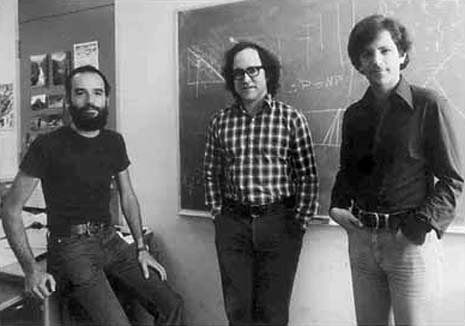
\includegraphics[width=0.75\textwidth]{./images/rsa.jpeg}
        \caption{Adi Shamir, Ronald Rivest, and Leonard Adelman}\label{fig:rsa}
\end{figure}

\section{RSA Algorithm}
\epigraphwidth=0.4\textwidth
\epigraph{\emph{The magic words are \emph{Squeamish Ossifrage}.}}{---Ronald L. Rivest}

\noindent The security of RSA relies on the practical difficulty of
factoring the product of two large prime numbers, known as the
\emph{factoring problem}. Breaking RSA encryption is known as the
\emph{RSA problem}. Whether it is as difficult as the factoring problem
is an open question. There are no published methods to defeat the system
if a large enough key is used, but RSA would be vulnerable to attack by
a \emph{quantum computer}.

RSA involves a public key and a private key. Everyone can know the
public key, and it is used for encrypting messages. The intention is
that messages encrypted with the public key can only be decrypted by
using the private key. The integers $n$ and $e$ represent the public
key. The private key is represented by the integer $d$.

The public key consists of the modulus $n$ and the public exponent $e$.
The private key consists of the private exponent $d$, which must be kept
secret; $p$, $q$, and $\varphi(n)$ must also be kept secret since they
are used to calculate $d$. In fact, $p$ and $q$ ($\varphi(n)$ is
calculated from them) can be discarded after $d$ has been computed.

We proceed by choosing two large random primes $p$ and $q$, these
numbers must be kept secret. We then publish the number $n = p q$. You
might wonder why we can do this, and the reason is that it is
\emph{believed} to be hard to factor large composite integers into their
constituent primes. The \emph{fundamental theorem of arithmetic} tells
us that every integer has a \emph{unique} prime factorization.

Choose a \emph{random} integer $2 < e < n \ni \gcd(e, \varphi(n)) = 1$,
where $\varphi(n) = (p-1)(q-1)$. $\gcd(a, b)$ indicates the greatest
common divisor of $a$ and $b$, which is commonly computed using Euclid's
algorithm, which is defined recursively as:
\[
\gcd(a, b) =
\begin{cases}
         a  & \text{if}\; a = b \\
         \gcd(a, b - a)  & \text{if}\; a < b \\
         \gcd(a - b, b) & \text{if}\; a > b \
\end{cases}
\]
though we can calculate it much more rapidly using division. A good
choice for $e$ is $2^{16} + 1 = 65537$. You will understand why---to
some extent---after you finish \S \ref{numthm}.
Here's a hint: How many $1$ bits are in that number?

The $\varphi$ function is called the \emph{totient} of $n$, and that
denotes the number of positive integers up to a given integer $n$ that
are relatively prime to $n$. Note that for any prime $p$, $\varphi(p) =
p - 1$, and so $\varphi(n) = \varphi(p q) = (p-1)(q-1)$. We can share
$e$ with impunity. We say that our \emph{public key} is the pair
$\langle e, n \rangle$.

We now calculate a unique secret integer $d\in \{0, \ldots, n-1\}$ such
that $d \times e \equiv 1 \pmod{\varphi(n)}$. How do we find this $d$?
It turns out that we have known how to do it for more than $2300$
years---we use an algorithm attributed to \emph{Euclid}. How is it that
we can easily calculate $d$ while our adversary cannot? We know a secret
that he does not: we know $\varphi(n)$ while he only knows $n$. We call
$d$ our \emph{private key}.

We now define two functions: $D(m) = m^e \pmod{n}$ and $E(c) = c^d
\pmod{n}$. We will show in \S\ref{proof} that $\forall m \in \{0,
\ldots, n-1\}$ that $D(E(m)) = E(D(m)) = m$. Since $D$ and $E$ are
\emph{mutual inverses} and this will enable us to perform not only
encryption but also digital signatures.

\section{Mathematics of RSA}\label{proof}

\epigraphwidth=0.7\textwidth
\epigraph{\emph{If $\,{\cal P} = \NNP$, then all of modern cryptography collapses. On this happy thought\ldots}}{Michael O.\xspace Rabin, November 1998}

\noindent
The mathematics of RSA are based on arithmetic in a group of integers
modulo $n$, denoted $\mathbb{Z}/n$. This is the set $\{ 0, \ldots, n - 1
\}$ and all sets that are isomorphic to it. For example, $\{ n, \ldots,
2n -1 \} \pmod{n} = \{ 0, \ldots, n - 1 \} \pmod{n}$, and there are an
infinite number of such sets. Since they are \emph{all the same} we will
only concern ourselves with the one with the smallest numbers.  What do
we mean when we say that are the same? We mean that if $x \equiv k
\pmod{n}$ then $a n + x \equiv k \pmod{n}, \forall a \ge 0, a \in
\mathbb{Z}$. In other words, additional integer products of $n$ do not
matter.

The Euler-Fermat theorem says that if $a\in\mathbb{N}$ and
$n\in\mathbb{N}$ are \emph{coprime}, that is $\gcd(a, n) = 1$, then
$$a^{\varphi(n)} \equiv 1 \pmod{n}.$$ This will allow us, for example,
to take a message $M$ and have $M^{\varphi(n)} \equiv 1 \pmod{n}$.

What is $\varphi(n)$? It is the Euler totient function, and gives the
number of positive integers than that or equal to $n$ that are
relatively prime to $n$. For any prime number $p$,
$$
\varphi(p) = p - 1.
$$

For the RSA algorithm, we choose two large primes $p$ and $q$, and we
make $n = p q$. What does this mean for us with respect to $\varphi(n)$?
\begin{align*}
        \varphi(n) & = \varphi(p) \times \varphi(q) \\
        & = (p - 1) (q - 1) \\
        & = n - (p + q) + 1 .
\end{align*}

We choose an encryption key $e$ such that is it relatively prime to
$\varphi(n)$, that is, $\gcd(e, \varphi(n)) = 1$. We can then deduce our
decryption key $d$ such that $e \times d \equiv 1 \pmod{\varphi(n)}$.
Our encryption algorithm is simply $E(M) = M^e \pmod{n} = C$, and our
decryption algorithm is $D(C) = c^d \pmod{n} = M$.

We have the additional property of being mutual inverses:
$E(D(x)) = D(E(x)) = x$,
and that will give us the ability to provide \emph{digital signatures}.
Observe that,
\begin{align*}
        D(E(M)) &\equiv E(M)^d \equiv M^{e d} \pmod{n} \\
        E(D(M)) &\equiv D(M)^e \equiv M^{d e} \pmod{n}.
\end{align*}
Continuing in this manner, observe that,
\[
  M^{e d} \equiv M^{k \varphi(n) + 1} \pmod{n}
\]
for some multiplier $k \ge 1$. This is true because, prior to the
modular reduction, $ed$ must be one greater than some multiple of
$\varphi(n)$; applying the modulus is what makes
$e d \equiv 1 \pmod{\varphi(n)}$. We can rewrite this as
\[
  M^{e d} \equiv (M^{\varphi(n)})^k \times M \pmod{n}.
\]
Here we apply Euler's theorem, which states that if $a$ and $n$ are
coprime integers, then $a^{\varphi(n)} \equiv 1 \pmod{n}$. So, assuming
that $M$ is coprime with $n$, we can simplify the above equation to
\begin{align*}
  M^{e d} &\equiv (1)^k \times M  &&\pmod{n} \\
          &\equiv (1) \times M  &&\pmod{n} \\
          &\equiv M  &&\pmod{n}
\end{align*}
which shows that the encryption and decryption functions are
mutual inverses.

In practice, Carmichael's function can be used in place of Euler's totient in
the computation of the RSA key pair. Carmichael's function is denoted with
$\lambda(n)$, where $\lambda(n) = \operatorname{lcm}(\lambda(p), \lambda(q))$.
We indicate the least common multiple of some $a$ and $b$ with
$\operatorname{lcm}(a, b)$. From the definition of the least common multiple, we
see that
\begin{align*}
  \lambda(n) &= \lambda(pq) \\
             &= \operatorname{lcm}(\lambda(p), \lambda(q)) \\
             &= \frac{|\lambda(p) \times \lambda(q)|}{\operatorname{gcd}(\lambda(p), \lambda(q))}.
\end{align*}
If $p$ and $q$ are prime, then we know
$\lambda(p) = \varphi(p) = p - 1$, and $\lambda(q) = \varphi(q) = q - 1$. Thus,
\begin{align*}
  \lambda(n) &= \frac{|\lambda(p) \times \lambda(q)|}{\operatorname{gcd}(\lambda(p), \lambda(q))} \\
             &= \frac{|\varphi(p) \times \varphi(q)|}{\operatorname{gcd}(p - 1, q - 1)} \\
             &= \frac{|\varphi(n)|}{\operatorname{gcd}(p - 1, q - 1)}.
\end{align*}
It should be clear from this that $\varphi(n)$ is a multiple of $\lambda(n)$.
Therefore,
\begin{align*}
  M^{e d} &\equiv (M^{\varphi(n)})^k \times M &&\pmod{n} \\
          &\equiv (M^{j \times \lambda(n)})^k \times M &&\pmod{n} \\
          &\equiv (M^{\lambda(n)})^{jk} \times M &&\pmod{n}
\end{align*}
for some multiplier $j \ge 1$.

From Carmichael's generalization of Euler's theorem, we know that
$a^{\lambda(n)} \equiv 1 \pmod{n}$. Thus,
\begin{align*}
  M^{e d} &\equiv (M^{\lambda(n)})^{jk} \times M &&\pmod{n} \\
          &\equiv (1)^{jk} \times M  &&\pmod{n} \\
          &\equiv (1) \times M  &&\pmod{n} \\
          &\equiv M  &&\pmod{n},
\end{align*}
which demonstrates how $\lambda(n)$ can be used in place of $\varphi(n)$ for the
computation of the RSA key pair. For your assignment, you will be using
Carmichael's function when computing your RSA key pair.

\section{Your Task}

\epigraphwidth=0.5\textwidth
\epigraph{\emph{The people will believe what the media tells them they
believe.}}{---George Orwell}

\noindent
\begin{itemize}
  \item Initialize your Bloom filter and hash table.
  \item Read in a list of \emph{badspeak} words with \texttt{fscanf()}.
    Again, badspeak is simply oldspeak without a newspeak translation.
    Badspeak is strictly forbidden. Each badspeak word should be added
    to the Bloom filter and the hash table. The list of proscribed words
    will be in \texttt{badspeak.txt}, which can be found in the
    \texttt{resources} repository.
  \item Read in a list of \emph{oldspeak} and \emph{newspeak} pairs with
    \texttt{fscanf()}. Only the oldspeak should be added to the Bloom
    filter. The oldspeak \emph{and} newspeak are added to the hash
    table. The list of oldspeak and newspeak pairs will be in
    \texttt{newspeak.txt}, which can also be found in the
    \texttt{resources} repository.
  \item Now that the lexicon of badspeak and oldspeak/newspeak
    translations has been populated, you can start to filter out words.
    Read words in from \texttt{stdin} using the supplied parsing module.
  \item For each word that is read in, check to see if it has been added
    to the Bloom filter. If it has not been added to the Bloom filter,
    then no action is needed since the word isn't a proscribed word.
  \item If the word has most likely been added to the Bloom filter,
    meaning \texttt{bf\_probe()} returned \texttt{true}, then further
    action needs to be taken.
    \begin{enumerate}
      \item If the hash table contains the word and the word \emph{does
        not} have a newspeak translation, then the citizen who used this
        word is guilty of \texttt{thoughtcrime}. Insert this badspeak
        word into a list of badspeak words that the citizen used in
        order to notify them of their errors later. What data structure
        could be used to store these words?
      \item If the hash table contains the word, and the word \emph{does}
        have a newspeak translation, then the citizen requires
        counseling on proper \emph{Rightspeak}. Insert this oldspeak
        word into a list of oldspeak words with newspeak translations in
        order to notify the citizen of the revisions needed to be made
        in order to practice Rightspeak.
      \item If the hash table does not contain the word, then all is
        good since the Bloom filter issued a false positive. No
        disciplinary action needs to be taken.
    \end{enumerate}
  \item If the citizen is accused of thoughtcrime \emph{and} requires
    counseling on proper \emph{Rightspeak}, then they are given a
    reprimanding \emph{mixspeak message} notifying them of their
    transgressions and promptly sent off to \emph{joycamp}. The message
    should contain the list of badspeak words that were used followed by
    the list of oldspeak words that were used with their proper newspeak
    translations.

  \begin{shlisting}{}
Dear beloved citizen of the GPRSC,

We have some good news, and we have some bad news.
The good news is that there is bad news. The bad news is that you will
be sent to joycamp and subjected to a week-long destitute existence.
This is the penalty for using degenerate words, as well as using
oldspeak in place of newspeak. We hope you can correct your behavior.

Your transgressions, followed by the words you must think on:

kalamazoo
antidisestablishmentarianism
write -> papertalk
sad -> happy
read -> papertalk
music -> noise
liberty -> badfree\end{shlisting}

  \item If the citizen is accused solely of thoughtcrime, then they are
    issued a thoughtcrime message and also sent off to \emph{joycamp}.
    The \emph{badspeak message} should contain the list of badspeak
    words that were used.

  \begin{shlisting}{}
Dear beloved citizen of the GPRSC,

You have been caught using degenerate words that may cause
distress among the moral and upstanding citizens of the GPSRC.
As such, you will be sent to joycamp. It is there where you will
sit and reflect on the consequences of your choice in language.

Your transgressions:

kalamazoo
antidisestablishmentarianism\end{shlisting}

  \item If the citizen only requires counseling, then they are issued an
    encouraging \emph{goodspeak message}. They will read it, correct
    their \emph{wrongthink}, and enjoy the rest of their stay in the
    GPRSC. The message should contain the list of oldspeak words that
    were used with their proper newspeak translations.

    \begin{shlisting}{}
Dear beloved citizen of the GPRSC,

We recognize your efforts in conforming to the language standards
of the GPSRC. Alas, you have been caught uttering questionable words
and thinking unpleasant thoughts. You must correct your wrongspeak
and badthink at once. Failure to do so will result in your deliverance
to joycamp.

Words that you must think on:

write -> papertalk
sad -> happy
read -> papertalk
music -> noise
liberty -> badfree\end{shlisting}

  \item Each of the messages are defined for you in \texttt{messages.h}.
    \textcolor{red}{You may not modify this file}.

  \item The list of the command-line options your program must support
    is listed below. \emph{Any} combination of the command-line options
    must be supported.
    \begin{itemize}
      \item \texttt{-h} prints out the program usage. Refer to the
      reference program in the resources repository for what to print.
      \item \texttt{-t size} specifies that the hash table
        will have \texttt{size} entries (the default will be $2^{16}$).
      \item \texttt{-f size} specifies that the Bloom filter
        will have \texttt{size} entries (the default will be $2^{20}$).
      \item \texttt{-s} will enable the printing of statistics to
        \texttt{stdout}. The statistics to calculate are:
        \begin{itemize}
          \item Average binary search tree size
          \item Average binary search tree height
          \item Average branches traversed
          \item Hash table load
          \item Bloom filter load
        \end{itemize}
        The latter three statistics are computed as follows:
        \begin{align*}
          \text{Average branches traversed} &=
          \frac{\texttt{branches}}{\texttt{lookups}} \\
          \text{Hash table load} &= 100 \times \frac{\texttt{ht\_count()}}{\texttt{ht\_size()}} \\
          \text{Bloom filter load} &= 100 \times \frac{\texttt{bf\_count()}}{\texttt{bf\_size()}}
        \end{align*}
        The hash table load and Bloom filter load should be printed with
        up to 6 digits of precision. \textcolor{red}{Enabling the
        printing of statistics should \emph{suppress all messages} the
        program may otherwise print.} The number of lookups is defined
        as the number of times \texttt{ht\_lookup()} and
        \texttt{ht\_insert()} is called. The number of branches is
        defined as the count of links traversed during calls to
        \texttt{bst\_find()} and \texttt{bst\_insert()}. The global
        variable \texttt{lookups} should be defined in \texttt{ht.c} and
        the global variable \texttt{branches} should be defined in
        \texttt{bst.c}.
    \end{itemize}
\end{itemize}

\section{GNU Multiple Precision Arithmetic}
\epigraph{\emph{One reason you should not use web applications to do your computing is
that you lose control. It's just as bad as using a proprietary program. Do your own
computing on your own computer with your copy of a freedom-respecting program.
If you use a proprietary program or somebody else's web server, you're defenceless.}}{%
---Richard Stallman}

\noindent
As you should know by now, \textbf{C}, unlike languages like
\textbf{Python}, does not natively support arbitrary precision integers.
The security of RSA, however, relies on large integers. So, we elect to
use the GNU multiple precision arithmetic library, usually referred to
as GMP\@. You can find the manual and documentation for the library
here:
\centerline{\url{https://gmplib.org/manual}.}
Take some time to look through the manual, taking note of which
functions may be useful.

You will need to install both \texttt{gmp} and \texttt{pkg-config}. The
latter is a utility used to assist in finding and linking libraries,
instead of having the program hard-code where to find specific headers
and libraries during program compilation. To install these packages on
Ubuntu 20.04, run the following:

\begin{shlisting}{}
$ sudo apt install pkg-config libgmp-dev
\end{shlisting}

Get started on this \emph{as soon as possible}. Make sure to attend
section for assistance on using \texttt{pkg-config} in a
\texttt{Makefile} to direct the compilation process for your programs.

You may notice that GMP already provides number theoretic functions,
several of which \emph{could} be used in RSA. \textcolor{red}{You may
not use any GMP-implemented number theoretic functions. You \emph{must}
implement those functions yourself.}

The following two sections (\S6 and \S7) will present the functions that
you have to implement, but they both will require the use of random,
arbitrary-precision integers.

GMP requires us to explicitly initialize a random state variable and
pass it to any of the random integer functions in GMP\@. Not only that,
we also need to call a dedicated function to clean up any memory used by
the initialized random state. To remedy this, you will implement a small
random state module, which contains a single \texttt{extern} declaration
to a global random state variable called \texttt{state}, and two
functions: one to initialize the state, and one to clear it. The
interface for the module will be given in \texttt{randstate.h} and the
implementation must go in \texttt{randstate.c}.

\begin{funcdoc}{void randstate\_init(uint64\_t seed)}
  Initializes the global random state named \texttt{state} with a Mersenne
  Twister algorithm, using \texttt{seed} as the random seed. You should call
  \texttt{srandom()} using this seed as well. This function will also entail
  calls to \texttt{gmp\_randinit\_mt()} and to \texttt{gmp\_randseed\_ui()}.
\end{funcdoc}

\begin{funcdoc}{void randstate\_clear(void)}
  Clears and frees all memory used by the initialized global random
  state named \texttt{state}. This should just be a single call to
  \texttt{gmp\_randclear()}.
\end{funcdoc}

\section{Number Theoretic Functions}
\epigraph{\emph{No one has yet discovered any warlike purpose to be served by the theory of numbers or relativity, and it seems unlikely that anyone will do so for many years.}}
{---G.\xspace H.\xspace Hardy}

\noindent
Number Theory is the branch of mathematics that studies the nature
and properties of numbers. Though many have made important contributions
to the field, including Gau{\ss} in his \emph{Disquisitiones
Arithmeticae} (which he completed when he was 21 years old), the
most important for public-key cryptography are Fermat and Euler
(Figure\xspace\ref{fig:euler}).

You will first need to implement the functions that drive the
mathematics behind RSA before you can tackle your RSA library. The
interface for these functions will be given in \texttt{numtheory.h} and
should be defined in corresponding \textbf{C} file. Read each of the subsections
carefully to understand, on some level, the theory behind each of the
number theoretic functions. Pseudocode is provided to assist you.

\begin{figure}[tbhp]
        \centering
        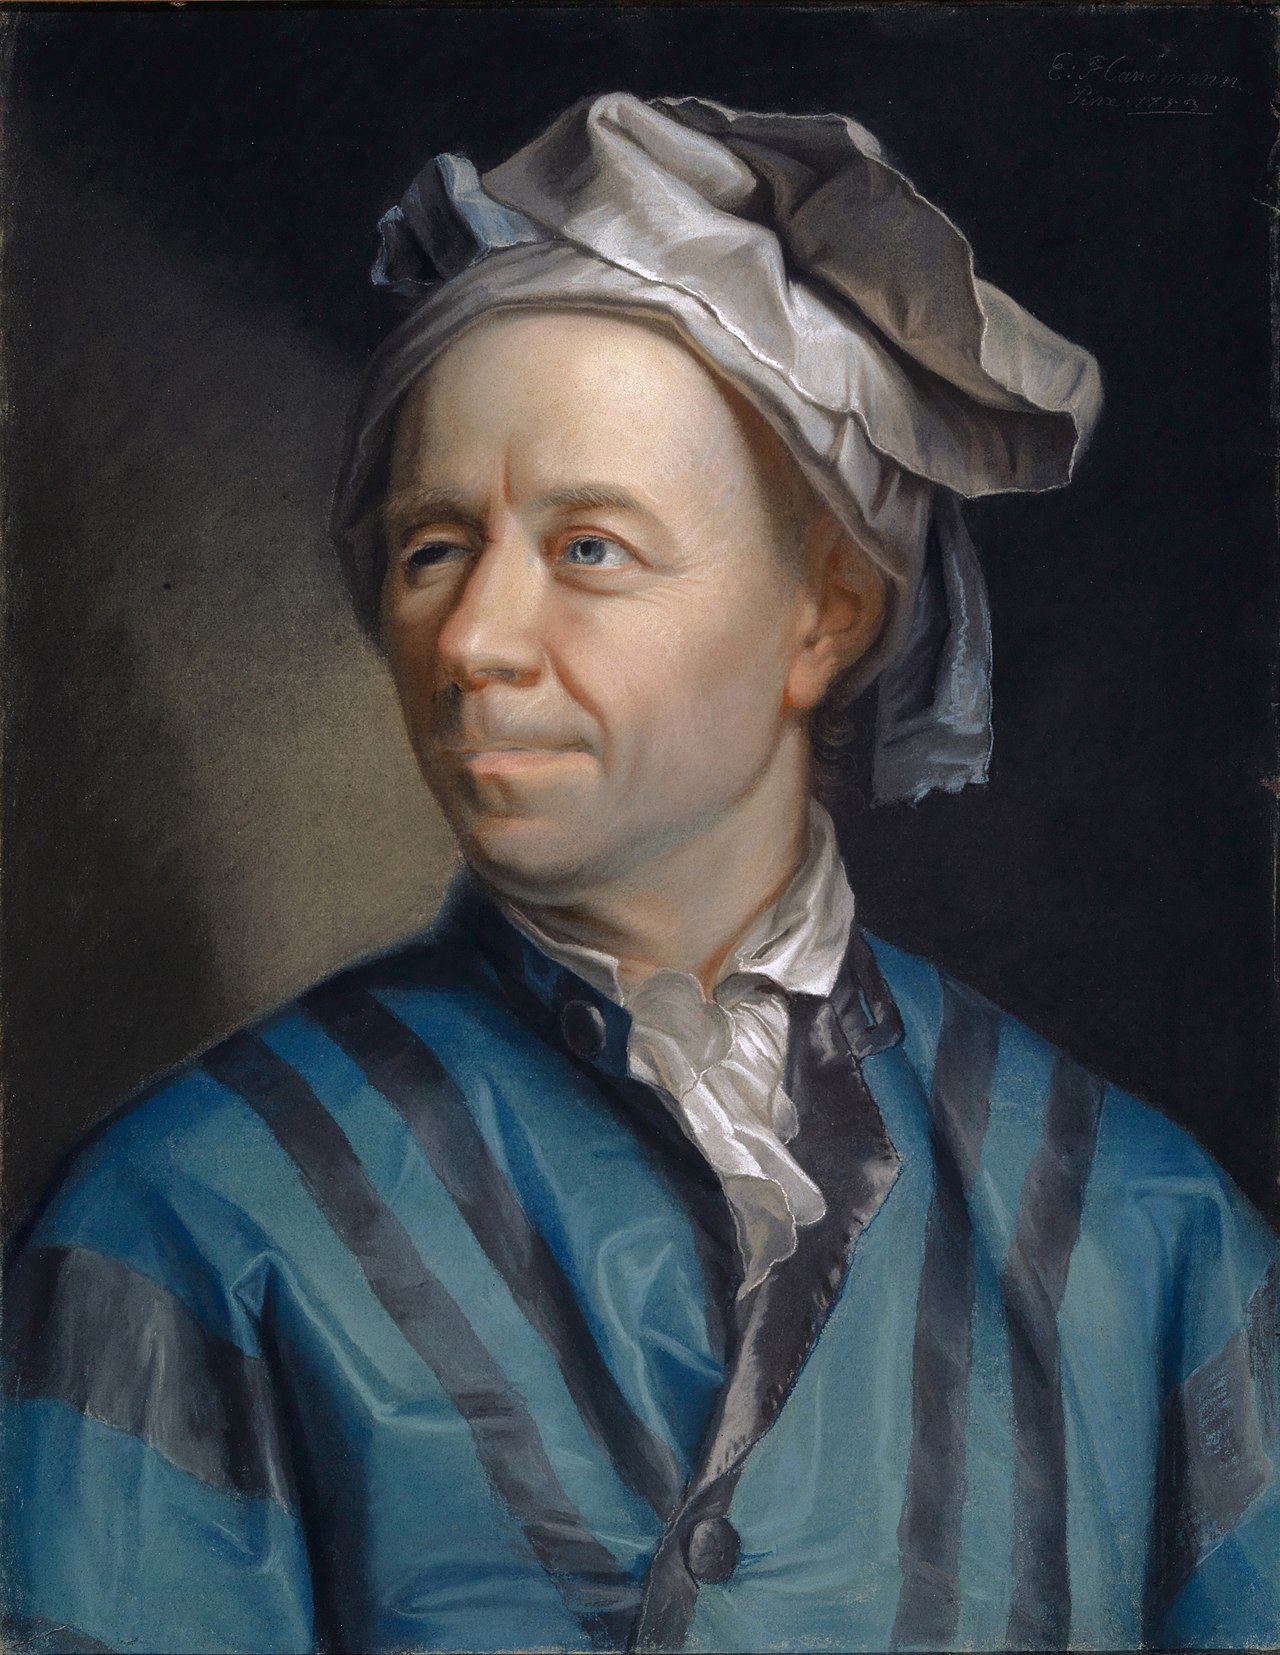
\includegraphics[height=0.23\textwidth]{./images/euler.jpg}\quad
        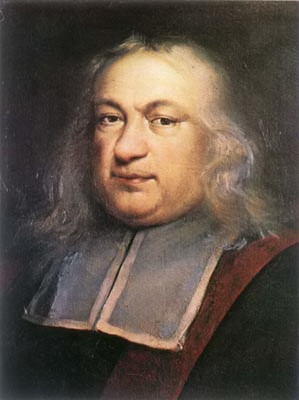
\includegraphics[height=0.23\textwidth]{./images/fermat.jpg}
        \caption{Leonhard Euler (1707--1783) and Pierre de Fermat (1607--1665)}\label{fig:euler}
\end{figure}
\subsection{Modular Exponentiation}

As shown in \S2, we must compute $a^n$ where both $a, n \in \mathbb{N}$
for RSA. We could simply multiply:
\[
  a^n = \overbrace{a \times a \times \cdots \times a \times a}^n .
\]
The number of multiplications is $n-1$,
which is ${O}(n)$. While correct, this approach is na{\"{i}}ve and
\emph{extremely inefficient}. Since we are working with very large
numbers in RSA, we must be able to compute modular exponentiation
quickly. So the question is, can we do better? We can in fact do much
better, computing $a^n$ in $\operatorname{O}(\log_2(n))$ steps.

Recall that we can write any integer as a polynomial
\[
  n = c_m 2^m + c_{m-1} 2^{m-1} + \cdots + c_1 2^1 + c_0 2^0 =
  \sum_{0\le i \le m} c_i 2^i ,
\]
where $n \ge 2^m$ and $c_i \in \{0, 1\}$. And so,
\[
  a^n = a^{c_m 2^m + c_{m-1} 2^{m-1} + \cdots + c_1 2^1 + c_0 2^0} .
\]
Since $a^{b+c} = a^b \times a^c$, then we can rewrite the formula as
\[
  a^n = a^{c_m 2^m} \times a^{c_{m-1} 2^{m-1}} \times \cdots \times
  a^{c_1 2^1} \times a^{c_0 2^0} = \prod_{0\le i \le m} a^{c_i 2^i} .
\]
As an example, consider $a^{13} = a^{2^3 + 2^2 + 2^0} = a^{8 + 4 + 1} =
a^8 \times a^4 \times a^1$. You will want to try a few more to get a
feeling for it before you attempt to write code.

This leaves us with the problem of computing the $a^{2^i}$ terms. We
start with $a = a^1$ and if we square it then $(a^1)^2 = a^2$. Each
time we square, $(a^2)^2 = a^4, (a^4)^2 = a^8, \ldots$ the exponents
are a power of $2$. We only have to square our previous result $\log_2
n$ times at most.

You will notice that the numbers get \emph{very large, very fast}.
Although we want enormous numbers for cryptography, we do not want
numbers that would be impossible to even write down if we used every
atom in the universe. Recall that $10^k$ is $k$ digits long. That
means that if $k=10^{1000}$ then there are that many digits (there are
approximately $10^{82}$ atoms in the observable universe).
Consequently, we will usually do such computations (mod ${n}$) for
some modulus $n$, meaning that all numbers are in $\{0, \ldots,
n-1\}$.

To implement modular exponentiation, you should simply follow the
steps to perform exponentiation by squaring as shown above and
reduce your results modulo $n$ after each operation that is likely to
yield a large result (you do not need to do it, if for example, you
just add a small constant). The following pseudocode shows the
repeated squaring and modular reduction at each step.

\begin{codebox}
  \Procname{\proc{Power-Mod}($a,d,n$)}
  \li $v \gets 1$
  \li $p \gets a$
  \li \While $d > 0$
  \li \Then \If \proc{Odd}(d)
  \li       \Then $v \gets (v \times p) \mod n$ \End
  \li       $p \gets (p \times p) \mod n$
  \li       $d \gets \lfloor d / 2 \rfloor$
      \End
  \li \Return $v$
\end{codebox}

The function that you are expected to implement to perform modular
exponentiation should be declared as follows:

\begin{funcdoc}{void pow\_mod(mpz\_t out, mpz\_t base, mpz\_t exponent,
  mpz\_t modulus)}
  Performs fast modular exponentiation, computing \texttt{base} raised
  to the \texttt{exponent} power modulo \texttt{modulus}, and storing
  the computed result in \texttt{out}.
\end{funcdoc}

\subsection{Primality Testing}
\epigraphwidth=0.6\textwidth
\epigraph{\emph{There are many methods---none of them as good as the randomized primality test.}}{---Michael O.\space Rabin, October 1997}


\noindent
The simplest primality test is trial division: given an input number,
$n$, check whether it is evenly divisible by any prime number between
$2$ and $\sqrt{n}$. Thus, this simple algorithm\footnote{
How big is $\sqrt{n}$? A typical encryption key has more than $600$ decimal digits. Thus,
$\sqrt{10^{600}}=10^{300}$.
Suppose we can do one trial division every \emph{nanosecond}, then that's $10^{300-9} = 10^{291}$ seconds. There are $22,896,000$ or about $10^7$ seconds per year, so it will take about $10^{284}$ years (the Big Bang was about $13.7\times 10^{9}$ years ago).
}
is $O(\sqrt{n})$,
but can we do better? The answer is subtle. To be certain,
we must try all of the primes from up to $\sqrt{n}$; there is no
way to escape it. But we can do much better if we are willing to
accept an answer of \emph{probably}.

Since it is infeasible to use a \emph{deterministic} algorithm, we
can solve many problems with \emph{high probability} by using a
\emph{randomized algorithm}. Such algorithms explore random parts
of the problem space so that we have high (but not perfect) confidence
that they have solved the problem.

Probabilistic tests are more rigorous than heuristic tests in that
they provide provable bounds on the probability of being fooled by
a composite number. All practical primality tests are probabilistic
tests. These tests use, apart from the tested number $n$, some other
number $a$ (called a \emph{witness}) that is chosen at random from
some sample space. The usual randomized primality tests never report
a prime number as composite, but a composite number may be reported
as prime.

The simplest probabilistic primality test is the Fermat primality
test. It works as follows: Given an integer $n$, choose some integer
a coprime to $n$ and calculate $a^{n - 1} \pmod{n}$. If the result
is different from $1$, then $n$ is composite. If it is $1$, then
$n$ may be prime. If $a^{n-1} \equiv 1 \pmod{n}$ $n$ is not prime,
then $n$ is called a pseudoprime to base $a$. In practice, we
observe that, if $a^{n-1} \equiv 1 \pmod{n}$, then $n$ is usually
prime.

Better yet is the Solovay-Strassen probabilistic primality test,
developed by Robert M.\xspace Solovay and Volker Strassen in 1977.
It is of particular importance since it made practical public-key
algorithms such as RSA.

\begin{figure}[tbhp]
\centering
  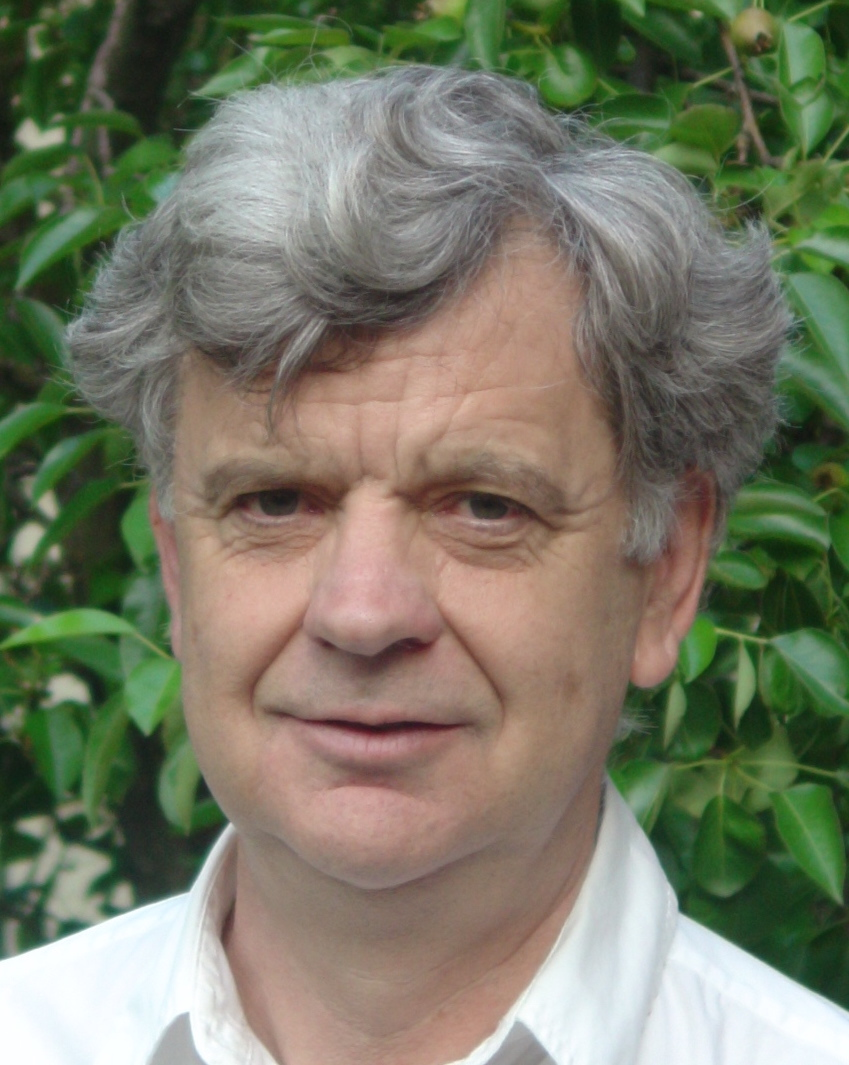
\includegraphics[height=0.33\textwidth]{./images/miller.jpg}\quad
  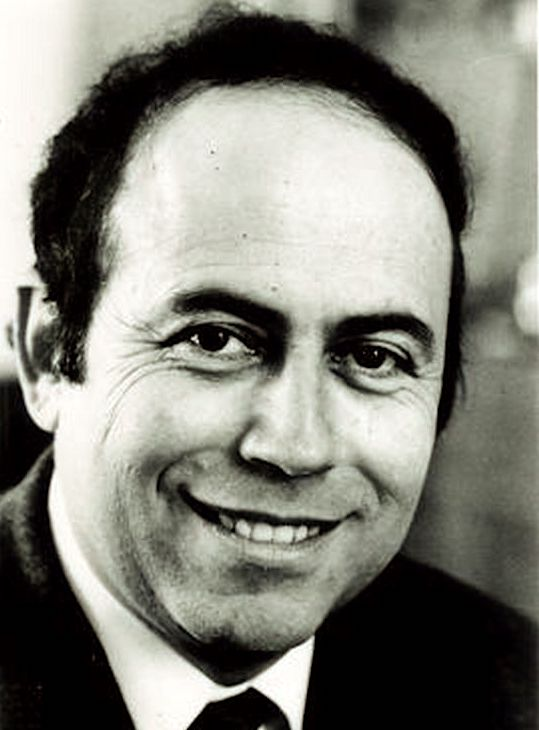
\includegraphics[height=0.33\textwidth]{./images/rabin.jpg}
\caption{Gary L.\xspace Miller and Michael O.\xspace Rabin}\label{fig:rabin}
\end{figure}

The Miller–Rabin primality test, invented by Gary Miller and Michael
O.\xspace Rabin (Figure\xspace\ref{fig:rabin}), is an even more
sophisticated probabilistic test, which detect all composites (once
again, this means: for every composite number $n$, at least
$\frac{3}{4}$ of numbers $a$ are witnesses of compositeness of $n$). The
accuracy of these tests is compared in Figure\xspace\ref{fig:tests}.

\begin{figure}[tbhp]
\centering
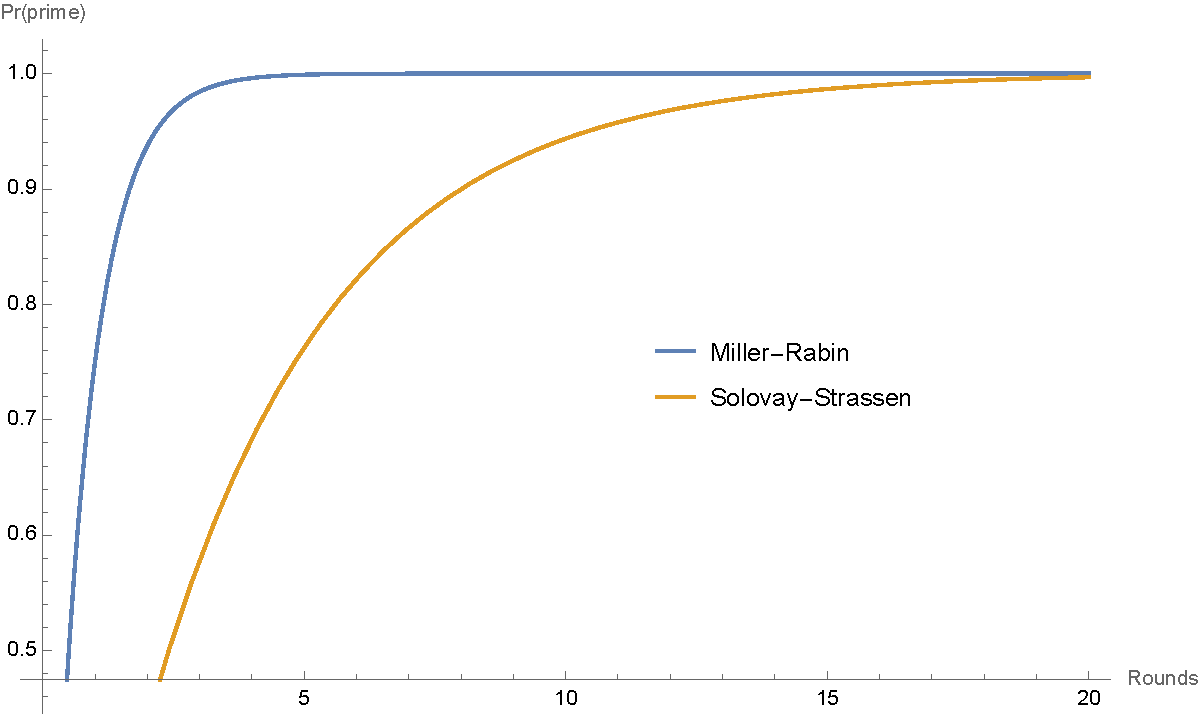
\includegraphics[width=0.75\textwidth]{./graphs/PrimeTest.pdf}
\caption{$\Pr[\text{prime}(p)]$ after successfully passing a given number of rounds.}\label{fig:tests}
\end{figure}

The Miller–Rabin primality test works as follows: Given an integer $n$,
choose some positive integer $a < n$. Let $2^s d = n - 1$, where $d$ is
odd. If $a^d \not\equiv \pm 1 \pmod{n}$ and $a^{{2^r} d} \not\equiv \pm
1 \pmod{n}$ for all $0 \le r \le s - 1$, then $n$ is composite and $a$
is a witness for the compositeness. Otherwise, $n$ \emph{might} be
prime. That is, we might be wrong $\frac{1}{4}$ of the time. If we
repeat the test $100$ times then our chance of being wrong is
$(\frac{1}{4})^{100} = 2^{-200}$ and that is usually more than good
enough. The Miller–Rabin test is considered a strong pseudoprime test,
where a pseudoprime is a number that is determined to be \emph{probably
prime} by a probabilistic test, but not actually prime. Deterministic
primality tests, such as the AKS primality test, do not give false
positives.

\begin{codebox}
  \Procname{\proc{Miller-Rabin}($n,k$)}
  \li write $n - 1 = 2^sr$ such that $r$ is odd
  \li \For $i \gets 1$ \To $k$
  \li \Then choose random $a \in \{\,2,3,\dots,n-2\,\}$
  \li       $y = \proc{Power-Mod}(a, r, n)$
  \li       \If $y \ne 1$ and $y \ne n - 1$
  \li       \Then $j \gets 1$
  \li             \While $j \le s - 1$ and $y \ne n - 1$
  \li             \Then $y \gets \proc{Power-Mod}(y, 2, n)$
  \li                   \If $y == 1$ \li \Then \Return \const{false} \End
  \li                   $j \gets j + 1$
                  \End
  \li             \If $y \ne n - 1$ \li \Then \Return \const{false} \End
            \End
      \End
  \li \Return \const{true}
\end{codebox}

The function that you are expected to implement to perform primality
testing should be declared as follows:

\begin{funcdoc}{bool is\_prime(mpz\_t n, uint64\_t iters)}
  Conducts the Miller-Rabin primality test to indicate whether or not
  \texttt{n} is prime using \texttt{iters} number of Miller-Rabin
  iterations. This function is needed when creating the two large primes
  $p$ and $q$ in RSA, verifying if a large integer is a prime.
\end{funcdoc}

In addition to the \texttt{is\_prime()} function, you are also required
to implement the following function:

\begin{funcdoc}{void make\_prime(mpz\_t p, uint64\_t bits, uint64\_t
  iters)}
  Generates a new prime number stored in \texttt{p}. The generated prime
  should be at least \texttt{bits} number of bits long. The primality of
  the generated number should be tested using \texttt{is\_prime()} using
  \texttt{iters} number of iterations.
\end{funcdoc}

\subsection{Modular Inverses}

The Euclidean algorithm, also called  Euclid's algorithm, is an
efficient method for computing the greatest common divisor ($\gcd$) of
two integers, the largest number that divides them both with a zero
remainder. The Euclidean algorithm is based on the principle that the
greatest common divisor of two numbers does not change if their
difference replaces the larger number with the smaller number. Since
this replacement reduces the larger of the two numbers, repeating this
process gives successively smaller pairs of numbers until the two
numbers become equal. We can accomplish this much faster if we compute
the remainder, which is equivalent to subtracting the smaller number
from the larger until it is no longer larger. You will first want to
implement the following function to compute the greatest common divisor
of two integers, which should be defined as follows:

\begin{funcdoc}{void gcd(mpz\_t d, mpz\_t a, mpz\_t b)}
  Computes the greatest common divisor of \texttt{a} and \texttt{b},
  storing the value of the computed divisor in \texttt{d}.

  \begin{codebox}
    \Procname{\proc{gcd}($a,b$)}
    \li \While $b \ne 0$
    \li \Then $t \gets b$
    \li       $b \gets a \bmod b$
    \li       $a \gets t$
        \End
    \li \Return $a$
  \end{codebox}
\end{funcdoc}

The extended Euclidean algorithm is an extension to the Euclidean
algorithm, and computes, in addition to the greatest common divisor
(gcd) of integers a and b, also the coefficients of B\'ezout's identity,
which are integers $x$ and $y$ such that
\[
  a x + b y = \gcd(a, b) .
\]
The extended Euclidean algorithm is particularly useful when $a$ and $b$
are coprime. With that provision, $x$ is the modular multiplicative
inverse of $a \pmod{b}$, and $y$ is the modular multiplicative inverse
of $b \pmod{a}$.

B\'ezout's identity asserts that $a$ and $n$ are coprime if and only if
there exist integers $s$ and $t$ such that
\[
  n s + a t = 1.
\]
Reducing this identity modulo $n$ gives
\[
  a t \equiv 1 \pmod{n}.
\]
To adapt the extended Euclidean algorithm to the problem of computing
the multiplicative inverse, note that the B\'ezout coefficient of $n$ is
not needed and so does not need to be computed. Also, for getting a
positive and result that is less than $n$,  use the fact that the
integer $t$ provided by the algorithm satisfies $| t | < n$. That is, if
$t < 0$, add $n$ to it at the end.

\begin{codebox}
  \Procname{\proc{Mod-Inverse}($a,n$)}
  \li $(r, r') \gets (n, a)$
  \li $(t, t') \gets (0, 1)$
  \li \While $r' \ne 0$
  \li \Then $q \gets \lfloor r / r' \rfloor$
  \li       $(r, r') \gets (r', r - q \times r')$
  \li       $(t, t') \gets (t', t - q \times t')$
      \End
  \li \If $r > 1$ \li \Then \Return no inverse \End
  \li \If $t < 0$ \li \Then $t \gets t + n$ \End
  \li \Return $t$
\end{codebox}

The function that you are expected to implement to compute modular
inverses should be declared as follows:

\begin{funcdoc}{void mod\_inverse(mpz\_t i, mpz\_t a, mpz\_t n)}
  Computes the inverse \texttt{i} of \texttt{a} modulo \texttt{n}. In
  the event that a modular inverse cannot be found, set \texttt{i} to 0.
  Note that this pseudocode uses parallel assignments, which \textbf{C}
  \emph{does not} support. Thus, you will need to use auxiliary
  variables to fake the parallel assignments.
\end{funcdoc}
\label{numthm}
\section{An RSA Library}
\epigraph{\emph{If you think cryptography is the answer to your problem, then you don't know what your problem is.}}{---Peter G.\xspace Neumann}

\noindent
\begin{funcdoc}{void rsa\_make\_pub(mpz\_t p, mpz\_t q, mpz\_t n, mpz\_t e,
uint64\_t nbits, uint64\_t iters)}
  Creates parts of a new RSA public key: two large primes \texttt{p} and
  \texttt{q}, their product \texttt{n}, and the public exponent
  \texttt{e}.

  \begin{enumerate}
    \item Begin by creating primes \texttt{p} and \texttt{q} using
      \texttt{make\_prime()}. We first need to decide the number of bits
      that go to each prime respectively such that $\log_2(\texttt{n})
      \ge \texttt{nbits}$. Let the number of bits for \texttt{p} be a
                  random number in the range
                  $\left [\texttt{nbits}/{4}, (3 \times \texttt{nbits})/{4} \right )$.
                  The remaining bits will go to
      \texttt{q}. The number of Miller-Rabin iterations is specified by
      \texttt{iters}.
    \item Next, compute $\varphi(\texttt{n}) = (\texttt{p} -
      1)(\texttt{q} - 1)$.
    \item We now need to find a suitable public exponent \texttt{e}. In
      a loop, generate random numbers of around \texttt{nbits} using
      \texttt{mpz\_urandomb()}. Compute the \texttt{gcd()} of each
      random number and the computed totient. Stop the loop you have
      found a number coprime with the totient: that will be the public
      exponent.
  \end{enumerate}
\end{funcdoc}

\begin{funcdoc}{void rsa\_write\_pub(mpz\_t n, mpz\_t e, mpz\_t
s, char username[], FILE *pbfile)}
  Writes a public RSA key to \texttt{pbfile}. The format of a public key
  should be \texttt{n}, \texttt{e}, \texttt{s}, then the
  \texttt{username}, each of which are written with a trailing newline.
  The values \texttt{n}, \texttt{e}, and \texttt{s} should be written as
  \emph{hexstrings}. See the GMP functions for
  \href{https://gmplib.org/manual/Formatted-Output-Functions}{formatted
  output} for help with writing hexstrings.
\end{funcdoc}

\begin{funcdoc}{void rsa\_read\_pub(mpz\_t n, mpz\_t e, mpz\_t s,
char username[], FILE *pbfile)}
  Reads a public RSA key from \texttt{pbfile}. The format of a public
  should be \texttt{n}, \texttt{e}, \texttt{s}, then the
  \texttt{username}, each of which should have been written with a
  trailing newline. The values \texttt{n}, \texttt{e}, and \texttt{s}
  should have been written as \emph{hexstrings}. See the GMP functions
  for
  \href{https://gmplib.org/manual/Formatted-Input-Functions}{formatted
  input} for help with reading hexstrings.
\end{funcdoc}

% //
% // Generates the components for a new private RSA key.
% // Requires an accompanying RSA public key to complete the pair.
% // All mpz\_t arguments are expected to be initialized.
% //
% // d: will store the RSA private key.
% // e: the precomputed public exponent.
% // p: the first large prime from the public key generation.
% // p: the second large prime from the public key generation.
% //
\begin{funcdoc}{void rsa\_make\_priv(mpz\_t d, mpz\_t e, mpz\_t
p, mpz\_t q)}
  Creates a new RSA private key \texttt{d} given primes \texttt{p} and
  \texttt{q} and public exponent \texttt{e}. To compute \texttt{d},
  simply compute the inverse of \texttt{e} modulo $\varphi(n) =
  (\texttt{p} - 1)(\texttt{q} - 1)$.
\end{funcdoc}

\begin{funcdoc}{void rsa\_write\_priv(mpz\_t n, mpz\_t d, FILE
*pvfile)}
  Writes a private RSA key to \texttt{pvfile}. The format of a private key
  should be \texttt{n} then \texttt{d}, both of which are written with a
  trailing newline. Both these values should be written as hexstrings.
\end{funcdoc}

\begin{funcdoc}{void rsa\_read\_priv(mpz\_t n, mpz\_t d, FILE
*pvfile)}
  Reads a private RSA key from \texttt{pvfile}. The format of a private
  key should be \texttt{n} then \texttt{d}, both of which should have
  been written with a trailing newline. Both these values should have
  been written as \emph{hexstrings}.
\end{funcdoc}

\begin{funcdoc}{void rsa\_encrypt(mpz\_t c, mpz\_t m, mpz\_t e,
mpz\_t n)}
  Performs RSA encryption, computing ciphertext \texttt{c} by encrypting
  message \texttt{m} using public exponent \texttt{e} and modulus
  \texttt{n}. Remember, encryption with RSA is defined as $E(m) = c =
        m^e \pmod{n}$.
\end{funcdoc}

\begin{funcdoc}{void rsa\_encrypt\_file(FILE *infile, FILE *outfile,
mpz\_t n, mpz\_t e)}
  Encrypts the contents of \texttt{infile}, writing the encrypted
  contents to \texttt{outfile}. The data in \texttt{infile} should be in
  encrypted in \emph{blocks}. Why not encrypt the entire file? Because
  of \texttt{n}. We are working modulo \texttt{n}, which means that the
  value of the block of data we are encrypting must be strictly less
  than \texttt{n}. We have two additional restrictions on the values of
  the blocks we encrypt:
  \begin{enumerate}
    \item The value of a block cannot be 0: $E(0) \equiv 0 \equiv 0^e \pmod{n}$.
    \item The value of a block cannot be 1. $E(1) \equiv 1 \equiv 1^e \pmod{n}$.
  \end{enumerate}
  A solution to these additional restrictions is to simply
  \emph{prepend} a single byte to the front of the block we want to
  encrypt. The value of the prepended byte will be \texttt{0xFF}. This
  solution is not unlike the padding schemes such as PKCS and OAEP used
  in modern constructions of RSA\@. To encrypt a file, follow these
  steps:
  \begin{enumerate}
    \item Calculate the block size $k$. This should be
      $k = \lfloor(\log_2({\texttt{n}}) - 1) / 8\rfloor$.
    \item Dynamically allocate an array that can hold $k$ bytes. This
      array should be of type \texttt{(uint8\_t *)} and will serve as
      the block.
    \item Set the zeroth byte of the block to \texttt{0xFF}. This
      effectively prepends the workaround byte that we need.
    \item While there are still unprocessed bytes in \texttt{infile}:
      \begin{enumerate}
        \item Read at most $k - 1$ bytes in from \texttt{infile}, and
          let $j$ be the number of bytes actually read. Place the read
          bytes into the allocated block starting from index 1 so as to
          not overwrite the \texttt{0xFF}.
        \item Using \texttt{mpz\_import()}, convert the read bytes,
          including the prepended \texttt{0xFF} into an \texttt{mpz\_t
          m}. You will want to set the \texttt{order} parameter of
          \texttt{mpz\_import()} to \texttt{1} for most significant word
          first, \texttt{1} for the \texttt{endian} parameter, and
          \texttt{0} for the \texttt{nails} parameter.
        \item Encrypt \texttt{m} with \texttt{rsa\_encrypt()}, then
          write the encrypted number to \texttt{outfile} as a
          \emph{hexstring} followed by a trailing newline.
      \end{enumerate}
  \end{enumerate}
\end{funcdoc}

\begin{funcdoc}{void rsa\_decrypt(mpz\_t m, mpz\_t c, mpz\_t d,
mpz\_t n)}
  Performs RSA decryption, computing message \texttt{m} by decrypting
  ciphertext \texttt{c} using private key \texttt{d} and public modulus
  \texttt{n}. Remember, decryption with RSA is defined as $D(c) = m =
        c^d \pmod{n}$.
\end{funcdoc}

\begin{funcdoc}{void rsa\_decrypt\_file(FILE *infile, FILE *outfile,
mpz\_t n, mpz\_t d)}
  Decrypts the contents of \texttt{infile}, writing the decrypted
  contents to \texttt{outfile}. The data in \texttt{infile} should be
  decrypted in \emph{blocks} to mirror how \texttt{rsa\_encrypt\_file()}
  encrypts in blocks. To decrypt a file, follow these steps:
  \begin{enumerate}
    \item Calculate the block size $k$. This should be
      $k = \lfloor(\log_2({\texttt{n}}) - 1) / 8\rfloor$.
    \item Dynamically allocate an array that can hold $k$ bytes. This
      array should be of type \texttt{(uint8\_t *)} and will serve as
      the block.
    \item While there are still unprocessed bytes in \texttt{infile}:
      \begin{enumerate}
        \item Scan in a hexstring, saving the hexstring as a
          \texttt{mpz\_t c}. Remember, each block is written as a
          hexstring with a trailing newline when encrypting a file.
        \item Using \texttt{mpz\_export()}, convert \texttt{c} back into
          bytes, storing them in the allocated block. Let $j$ be the
          number of bytes actually converted. You will want to set the
          \texttt{order} parameter of \texttt{mpz\_export()} to
          \texttt{1} for most significant word first, \texttt{1} for the
          \texttt{endian} parameter, and \texttt{0} for the
          \texttt{nails} parameter.
        \item Write out $j - 1$ bytes starting from index 1 of the block
          to \texttt{outfile}. This is because index 0 must be prepended
          \texttt{0xFF}. Do not output the \texttt{0xFF}.
      \end{enumerate}
  \end{enumerate}

\end{funcdoc}

\begin{funcdoc}{void rsa\_sign(mpz\_t s, mpz\_t m, mpz\_t d, mpz\_t
n)}
  Performs RSA signing, producing signature \texttt{s} by signing
  message \texttt{m} using private key \texttt{d} and public modulus
        \texttt{n}. Signing with RSA is defined as $S(m) = s = m^d \pmod{n}$.
\end{funcdoc}

\begin{funcdoc}{bool rsa\_verify(mpz\_t m, mpz\_t s, mpz\_t e,
mpz\_t n)}
  Performs RSA verification, returning \texttt{true} if signature
  \texttt{s} is verified and \texttt{false} otherwise. Verification is
        the inverse of signing. Let $t = V(s) = s^e \pmod{n}$. The signature is
  verified if and only if $t$ is the same as the expected message
  \texttt{m}.
\end{funcdoc}

\section{Key Generator}
\epigraph{\emph{This method, seemingly very clever, actually played into our hands! And so it often happens that an apparently ingenious idea is in fact a weakness which the scientific cryptographer seizes on for his solution.}}{---Herbert Yardley, \emph{The American Black Chamber}}

\noindent
Your key generator program should accept the following command-line
options:
\begin{itemize}
  \item \texttt{-b}\,: specifies the minimum bits needed for the public
    modulus $n$.
  \item \texttt{-i}\,: specifies the number of Miller-Rabin iterations
    for testing primes (default: 50).
  \item \texttt{-n pbfile}\,: specifies the public key file (default:
    rsa.pub).
  \item \texttt{-d pvfile}\,: specifies the private key file (default:
    rsa.priv).
  \item \texttt{-s}\,: specifies the random seed for the random state
    initialization (default: the seconds since the \textsc{Unix} epoch,
    given by \texttt{time(NULL)}).
  \item \texttt{-v}\,: enables verbose output.
  \item \texttt{-h}\,: displays program synopsis and usage.
\end{itemize}

The program should follow these steps:
\begin{enumerate}
  \item Parse command-line options using \texttt{getopt()} and handle
    them accordingly.
  \item Open the public and private key files using \texttt{fopen()}.
    Print a helpful error and exit the program in the event of failure.
  \item Using \texttt{fchmod()} and \texttt{fileno()}, make sure that
    the private key file permissions are set to \texttt{0600},
    indicating read and write permissions for the user, and no
    permissions for anyone else.
  \item Initialize the random state using \texttt{randstate\_init()},
    using the set seed.
  \item Make the public and private keys using \texttt{rsa\_make\_pub()}
    and \texttt{rsa\_make\_priv()}, respectively.
  \item Get the current user's name as a string. You will want to use
    \texttt{getenv()}.
  \item Convert the username into an \texttt{mpz\_t} with
    \texttt{mpz\_set\_str()}, specifying the base as 62. Then, use
    \texttt{rsa\_sign()} to compute the signature of the username.
  \item Write the computed public and private key to their respective
    files.
  \item If verbose output is enabled print the following, each with a
    trailing newline, in order:
    \begin{enumerate}
      \item username
      \item the signature \texttt{s}
      \item the first large prime \texttt{p}
      \item the second large prime \texttt{q}
      \item the public modulus \texttt{n}
      \item the public exponent \texttt{e}
      \item the private key \texttt{d}
    \end{enumerate}
    All of the \texttt{mpz\_t} values should be printed with information
    about the number of bits that constitute them, along with their
    respective values in \emph{decimal}. See the reference key generator
    program for an example.
  \item Close the public and private key files, clear the random state
    with \texttt{randstate\_clear()}, and clear any \texttt{mpz\_t}
    variables you may have used.
\end{enumerate}

\section{Encryptor}
\epigraph{\emph{The laws of mathematics are very commendable, but the only law that
applies in Australia is the law of Australia.}}{---Malcolm Turnbull, Australian Prime Minister}

Your encryptor program should accept the following command-line options:
\begin{itemize}
  \item \texttt{-i}\,: specifies the input file to encrypt (default:
    \texttt{stdin}).
  \item \texttt{-o}\,: specifies the output file to encrypt (default:
    \texttt{stdout}).
  \item \texttt{-n}\,: specifies the file containing the public key
    (default: \texttt{rsa.pub}).
  \item \texttt{-v}\,: enables verbose output.
  \item \texttt{-h}\,: displays program synopsis and usage.
\end{itemize}
The program should follow these steps:
\begin{enumerate}
  \item Parse command-line options using \texttt{getopt()} and handle
    them accordingly.
  \item Open the public key file using \texttt{fopen()}. Print a helpful
    error and exit the program in the event of failure.
  \item Read the public key from the opened public key file.
  \item If verbose output is enabled print the following, each with a
    trailing newline, in order:
    \begin{enumerate}
      \item username
      \item the signature \texttt{s}
      \item the public modulus \texttt{n}
      \item the public exponent \texttt{e}
    \end{enumerate}
    All of the \texttt{mpz\_t} values should be printed with information
    about the number of bits that constitute them, along with their
    respective values in \emph{decimal}. See the reference encryptor
    program for an example.
  \item Convert the username that was read in to an \texttt{mpz\_t}.
    This will be the expected value of the verified signature. Verify
    the signature using \texttt{rsa\_verify()}, reporting an error and
    exiting the program if the signature couldn't be verified.
  \item Encrypt the file using \texttt{rsa\_encrypt\_file()}.
  \item Close the public key file and clear any \texttt{mpz\_t}
    variables you have used.
\end{enumerate}

\section{Decryptor}
\epigraphwidth=0.33\textwidth
\epigraph{\emph{So much technology, so little talent.}}{---Vernor Vinge, \emph{Rainbow's End}}

\noindent
Your decryptor program should accept the following command-line options:
\begin{itemize}
  \item \texttt{-i}\,: specifies the input file to decrypt (default:
    \texttt{stdin}).
  \item \texttt{-o}\,: specifies the output file to decrypt (default:
    \texttt{stdout}).
  \item \texttt{-n}\,: specifies the file containing the private key
    (default: \texttt{rsa.priv}).
  \item \texttt{-v}\,: enables verbose output.
  \item \texttt{-h}\,: displays program synopsis and usage.
\end{itemize}
The program should follow these steps:
\begin{enumerate}
  \item Parse command-line options using \texttt{getopt()} and handle
    them accordingly.
  \item Open the private key file using \texttt{fopen()}. Print a helpful
    error and exit the program in the event of failure.
  \item Read the private key from the opened private key file.
  \item If verbose output is enabled print the following, each with a
    trailing newline, in order:
    \begin{enumerate}
      \item the public modulus \texttt{n}
      \item the private key \texttt{e}
    \end{enumerate}
    Both these values should be printed with information about the
    number of bits that constitute them, along with their respective
    values in \emph{decimal}. See the reference decryptor program for an
    example.
  \item Decrypt the file using \texttt{rsa\_decrypt\_file()}.
  \item Close the private key file and clear any \texttt{mpz\_t}
    variables you have used.
\end{enumerate}

\section{Deliverables}

\epigraphwidth=0.4\textwidth
\epigraph{\emph{It is such a sweet temptation \\ It gives such grief relief \\
It is such a false sensation \\ How come that's so hard to believe?}}{---Ray
Wylie Hubbard, \emph{Loco Gringo's Lament}}

You will need to turn in the following source code and header files:

\begin{enumerate}
  \item Your program \emph{must} have the following source and header
    files:
  \begin{itemize}
    \item \texttt{universe.c} implements the \texttt{Universe} ADT.
    \item \texttt{universe.h} specifies the interface to the \texttt{Universe}
      ADT. This file is provided and \emph{may not} be modified.
    \item \texttt{life.c} contains \texttt{main()} and \emph{may}
      contain any other functions necessary to complete your implementation of
      the Game of Life.
  \end{itemize}
\end{enumerate}

You can have other source and header files, but \emph{do not try to be overly
clever}. You will also need to turn in the following:

\begin{enumerate}
  \item \texttt{Makefile}:
    \begin{itemize}
      \item \texttt{CC = clang} must be specified.
      \item \texttt{CFLAGS = -Wall -Wextra -Werror -Wpedantic} must be specified.
      \item \texttt{make} must build the \texttt{life} executable, as should
        \texttt{make all} and \texttt{make life}.
      \item \texttt{make clean} must remove all files that are compiler
        generated.
      \item \texttt{make format} should format all your source code,
        including the header files.
    \end{itemize}
  \item \texttt{README.md}: This must use proper Markdown syntax. It
    must describe how to use your program and \texttt{Makefile}. It
    should also list and explain any command-line options that your
    program accepts. Any false positives reported by \texttt{scan-build}
    should be documented and explained here as well. Note down any known
    bugs or errors in this file as well for the graders.
  \item \texttt{DESIGN.pdf}: This document \emph{must} be a proper
    PDF\@. This design document must describe your design and design
    process for your program with enough detail such that a sufficiently
    knowledgeable programmer would be able to replicate your
    implementation. \textcolor{red}{This does not mean copying your
    entire program in verbatim}. You should instead describe how your
    program works with supporting pseudocode.
  \item \texttt{WRITEUP.pdf}: This document \emph{must} be a proper
    PDF\@. This writeup document must include everything you learned from
    this assignment. Make sure to mention everything in detail while being as precise as possible. How well you explain all the lessons you have learned in this assignment will be really important here. 
\end{enumerate}

\section{Submission}

Refer back assignment 0 for the instructions on how to properly submit
your assignment through \texttt{git}. Remember: \emph{add},
\emph{commit}, and \emph{push}!

\textcolor{red}{Your assignment is turned in \emph{only} after you have
pushed and submitted the commit ID you want graded on Canvas. ``I
forgot to push'' and ``I forgot to submit my commit ID'' are not valid
excuses. It is \emph{highly} recommended to commit and push your changes
\emph{often}.}

\section{Supplemental Readings}

\epigraph{\emph{The more that you read, the more things you will know. The
more that you learn, the more places you'll go.}}{---Dr.\ Seuss}

\begin{itemize}
  \item \textit{The C Programming Language} by Kernighan \& Ritchie
  \begin{itemize}
    \item Chapter 7
    \item Appendix B
  \end{itemize}
  \item \textit{Introduction to Algorithms} by T.\ Cormen, C.\
    Leiserson, R.\ Rivest, \& C.\ Stein
    \begin{itemize}
      \item Chapter 31 \S 31.2, \S 31.3, \S 31.6, \S 31.7, \S 31.8
    \end{itemize}
\end{itemize}


\monkey{et ecce simia pallidus et qui nomen illi \textbf{\textit{C}}  et inferus sequebatur eum}

\end{document}
